\documentclass[12pt]{article}

\usepackage[margin=1in]{geometry}
	%changes default margins
\usepackage{subcaption} %subfigure
\usepackage{setspace}
\usepackage{multirow}
\usepackage{booktabs}
\doublespacing
	%\singlespacing,\onehalfspacing,\doublespacing can be set and everything thereafter will use that spacing. You can switch within the document as often as you wish
	
\usepackage{parskip}
%changes paragraphs to have an extra space and new indentation with paragraphs, rather than indenting every new paragraph. This is completely a stylistic choice and neither is better than the other.


\usepackage{mathtools,amssymb} %useful math stuff. there are a lot of ams* packages. If you have a math need, it's probably in there

	
	
%\usepackage{natbib}
%\usepackage{biblatex} %natbib is older and available from almost all journals, biblatex is not, but biblatex has more flexibility and options.

%\usepackage[natbib=true]{biblatex} %this often works and requires minimal changes 

%for biblatex you write \textcite{citekey} and \parencite{citekey}
%for natbib you write \citet{citekey} and \citep{citekey}. Please avoid using \cite{} since you won't control whether it's parenthetical, but you are responsible for whether you use something in text or parenthetically.
%for \usepackage[natbib=true]{biblatex} you follow the natbib style and you won't have to perform search/replaces in your document, you would only need to change the package call and bibliography call.

\usepackage{natbib}
\bibliographystyle{chicago}

%other useful packages
% \usepackage{graphicx} %for including images including pdf



\title{Ast3: Death's End}
%\author{jsp ci 843503,\\ 
%	eswst i; ,i;l 830097,\\ 
%sjsms ,ovjs; 839866}
\author{
Hao Xu T00732492,\\
Waqar Ul Mulk T00729986,\\
Ahana Michael T00728755}
\date{\today}

\begin{document}
	
\maketitle

\section{Question 1}

\textbf{Because your response is binary (0 or 1), and you are modelling its expected value, what is your kernel smoother actually modelling? Hint: one of two words, both of which start with p.}

\underline{Probability}

\[
P(\text{isGentoo}=1 \mid \mathbf{x}_0) = \hat{f}(\mathbf{x}_0) = \frac{\sum_{i=1}^{N} K_{Type, \lambda}\left( \mathbf{x}_0, \mathbf{x}_i \right) y_i}{\sum_{i=1}^{N} K_{Type,\lambda}\left( \mathbf{x}_0, \mathbf{x}_i \right)}
\] 

Where $\mathbf{x}_0$ is a new data point in the test dataset, $N$ is the size of training data set, $K_{Type, \lambda}$ is the kernel function, and $\lambda$ is the bandwidth, $y_i$ represent the label of the $i^{\text{th}}$ training data.

\section{Question 2}

We implemented 2 different types of kernels: Box and Triangle. 

\begin{align*}
K_{\text{Box}, \lambda}(\mathbf{x}_0, \mathbf{x}_i) &= 
\begin{cases}
1, &\quad d_{*}(\mathbf{x}_0, \mathbf{x}_i)<\lambda\\
0, &\quad \text{otherwise}\\
\end{cases}\\
K_{\text{Triangle}, \lambda}(\mathbf{x}_0, \mathbf{x}_i) &= 
\begin{cases}
\frac{\lambda - d_{*}(\mathbf{x}_0, \mathbf{x}_i)}{\lambda}, &\quad d_{*}(\mathbf{x}_0, \mathbf{x}_i)<\lambda\\
0, &\quad \text{otherwise}\\
\end{cases}
\end{align*}

Where $d_{*}$ represent different types of distance metric: $d_{*} = d_{1}$ represent the $L_1$ (Manhattan) distance and $d_{*} = d_{2}$ represent the $L_2$ (Euclidean) distance.

%$L_1$ (Manhattan) distance between $\mathbf{a}=(a_1,a_2,a_3,a_4)$ and $\mathbf{b}=(b_1,b_2,b_3,b_4)$:
%\[
%d_{1}(\mathbf{a},\mathbf{b})=|a_1-b_1|+|a_2-b_2|+|a_3-b_3|+|a_4-b_4|
%.\] 
%
%$d_{*} = d_{2}$ represent the $L_2$ (Euclidean) distance between $\mathbf{a}=(a_1,a_2,a_3,a_4)$ and $\mathbf{b}=(b_1,b_2,b_3,b_4)$:
%\[
%d_{2}(\mathbf{a},\mathbf{b})=\sqrt{\left( a_1-b_1 \right) ^2+\left( a_2-b_2 \right) ^2+\left( a_3-b_3 \right) ^{2}+\left( a_4-b_4 \right) ^{2}} 
%.\] 

The output of our model is as follows:
\[
\text{Prediction}(\mathbf{x}_0)= 
\begin{cases}
1, &\quad P(\text{isGentoo}=1 \mid \mathbf{x}_0) = \hat{f}(\mathbf{x}_0) \ge 0.5\\
0, &\quad \text{otherwise}\\
\end{cases}
\]
If the probability of $\mathbf{x}_0$ to be Gentoo is greater than 50\%, we say it is Gentoo. \footnote{Here, this 50\% threshhold is arbitrarily selected. Theoratically, this threshhold can be any value in $\left( 0,1 \right) $ because we can use $\lambda$ to control the number of data points we included in our kernel. A lower threshold will result in a smaller $\lambda$ to get the best accuracy, vice versa.}

Not creating a training/test partition is a bad idea because we can always use a very small $\lambda$ to achieve 100\% training accuracy\footnote{This is because no matter how unreasonably small the $\lambda$ is, we always have one correct data point $\mathbf{x}_0$ selected by our kernel.}. Therefore, we use 10-fold cross validation to train and test our data. We define our training score as the average of test error rates across all 10 folds as follows: ($N_i$ is the $i^{\text{th}}$ test partition)
\[
\text{ERROR}_{Type,\lambda,d} = \left(\sum_{i=1}^{10}  \frac{\sum_{j\in N_i} \text{err}(j)}{|N_i|} \right) \cdot \frac{1}{10}, \quad \text{err}(j)=
\begin{cases}
1, &\quad \text{Prediction}\left(\mathbf{x}_j \right) \neq y_j\\
0, &\quad \text{otherwise}\\
\end{cases}\\
\] 

\begin{figure}[htbp]
\centering
\begin{subfigure}{0.6\textwidth}
    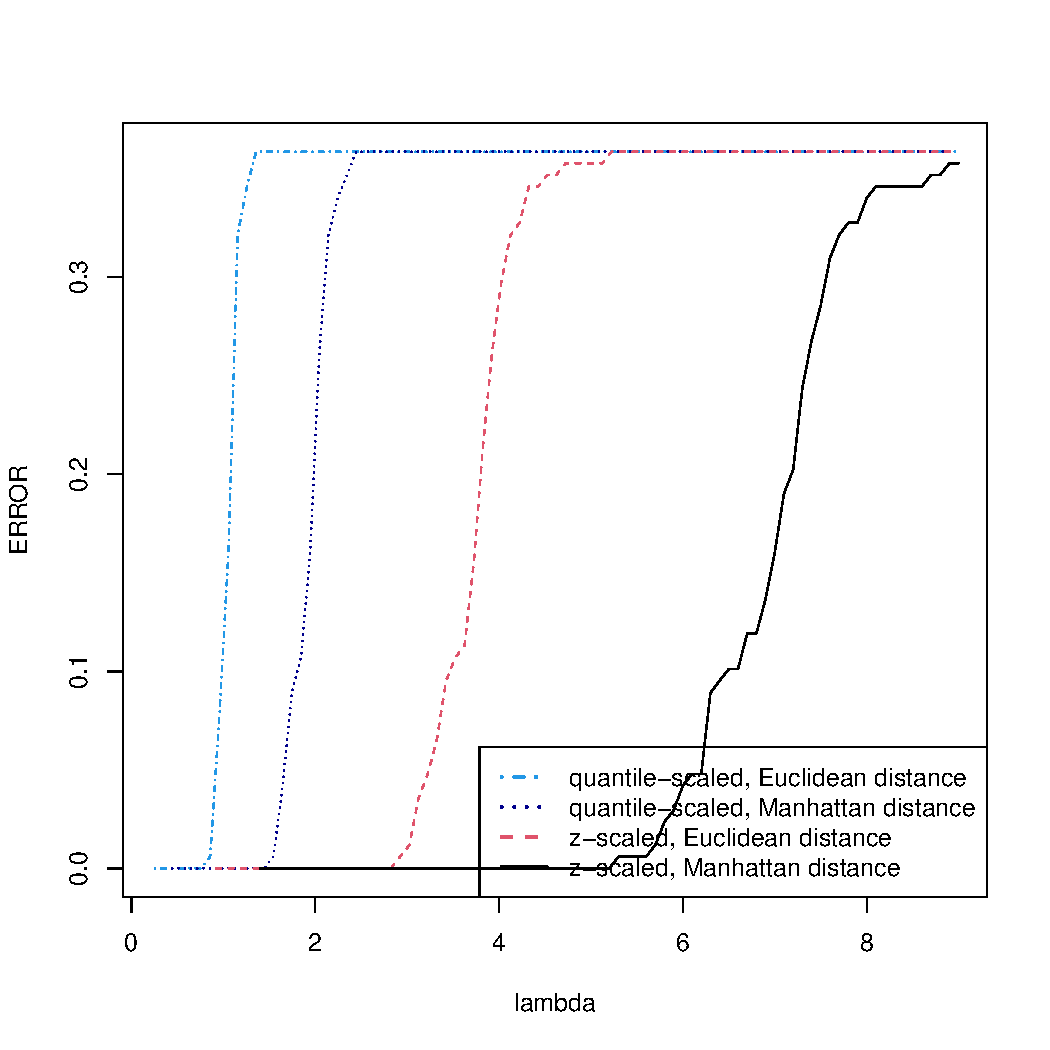
\includegraphics[width=\textwidth]{ERROR-lambda}
    \caption{Box Kernel}
    \label{fig:first}
\end{subfigure}
\hfill
\begin{subfigure}{0.6\textwidth}
    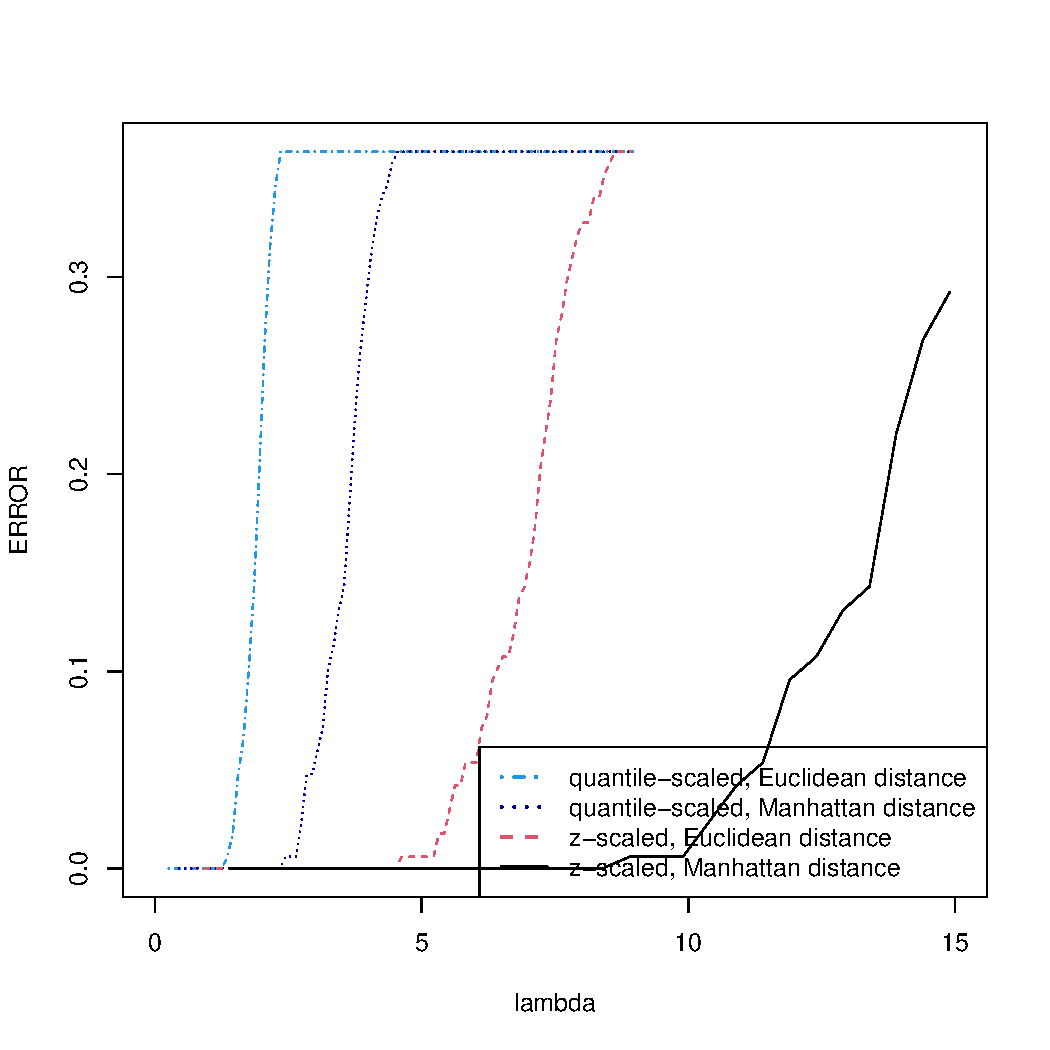
\includegraphics[width=\textwidth]{ERROR-lambda2}
    \caption{Triangle Kernel}
    \label{fig:second}
\end{subfigure}
        
\caption{ERROR-$\lambda$ plot}
\label{fig:result}
\end{figure}

The average test error rates depends on (1) the kernel bandwidth $\lambda$, (2) the type of distance metric and (3) the type of Kernel. Figure~\ref{fig:result} plots the ERROR--$\lambda$ relation. Box Kernel is used in figure~\ref{fig:first} and Triangle Kernel is used in figure~\ref{fig:second}. Comparing those figures, we can see that quantile scaled data requires a smaller $\lambda$, whereas z-scored scaled data requires a relative larger $\lambda$. Also Manhattan distance metric requires a relative larger $\lambda$ compares to Euclidean distance.

Additionally, we can see that Triangle Kernel performs more stable than Box Kernel (More tolerance to changes in $\lambda$).

\end{document}

